\subsection{Client}
\subsubsection{Diagramma di classe per l'unità}

\begin{figure}[H]
	\centering
	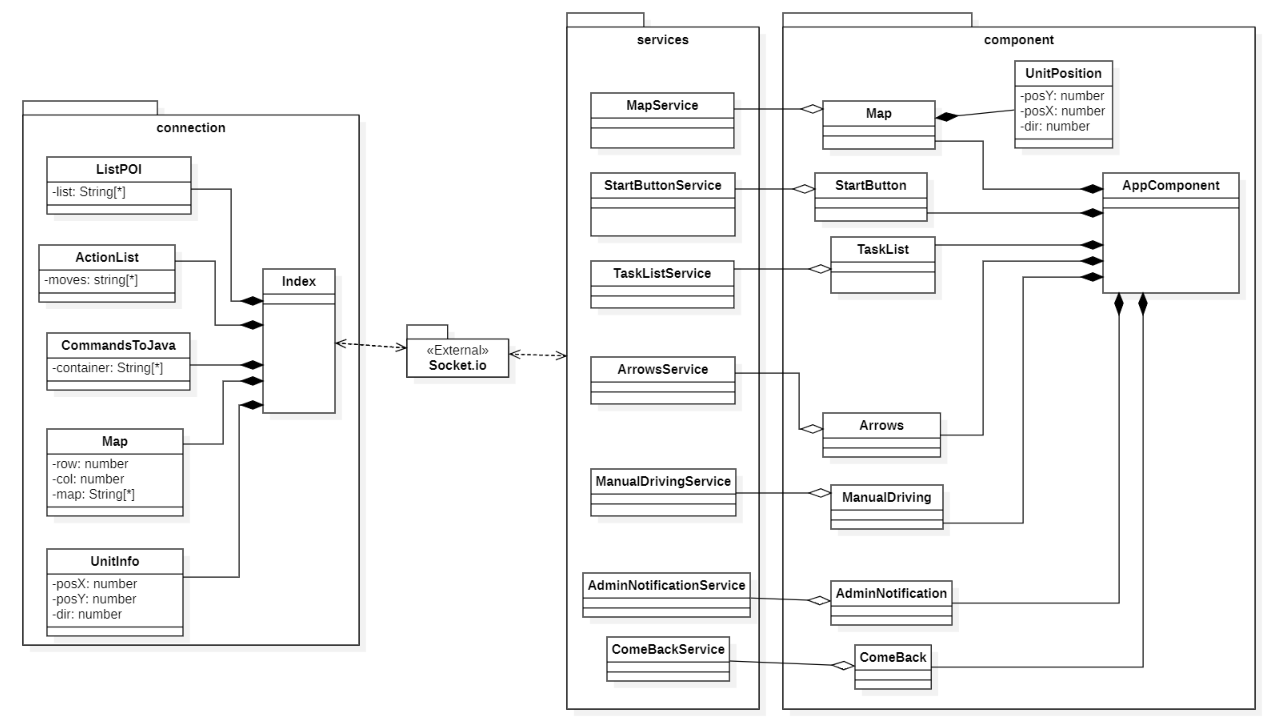
\includegraphics[scale=0.5]{res/images/UML_operatore.png}
	\caption{Diagramma UML delle classi per l'unità}
\end{figure}

Qui utilizziamo due tecnologie: Node per quanto riguarda il package connection e Angular per il resto. Queste due parti del front end comunicano attraverso il package esterno Socket.io, necessario gestire un flusso di dati attraverso i socket.\\
Il package services, come descritto anche nella documentazione di Angular, fa da intermediario tra il package connection e il package component, utilizzando degli Observer in ascolto di uno specifico socket e instradando l'informazione verso l'opportuno component.\\
Il package component permette di visualizzare sullo schermo le informazioni richieste grazie anche ai template di Angular. Ogni classe di questo package serve ad una specifica funzionalità:
\begin{itemize}
	\item \texttt{Map} → visualizza la mappa del magazzino con la posizione in real time dell'unità;
	\item \texttt{StartButton} → mostra un bottone che serve a far partire l'unità;
	\item \texttt{TaskList} → mostra la lista di task che l'operatore dovrà compiere;
	\item \texttt{Arrows} → visualizza le azioni che compie l'unità in real time;
	\item \texttt{ManualDrive} → permette di cambiare guida da manuale ad automatica e viceversa, facendo visualizzare anche i pulsanti da premere per far muovere l'unità manualmente in caso;
	\item \texttt{AdminNotification} → visulizza un pulsante che, se premuto, notifica all'admin un evento eccezionale;
	\item \texttt{ComeBack} → mostra un pulsante alla fine del turno dell'operatore che, se premuto, guida automaticamente il muletto verso la propria base.
\end{itemize}
Il package connection, attraverso le classi Index e CommandsToJava, instaura inoltre una comunicazione TCP Socket con java, permettendo di creare una connessione tra frontend e backend.\\

\subsubsection{Diagramma di classe per l'admin-manager}

\begin{figure}[H]
	\centering
	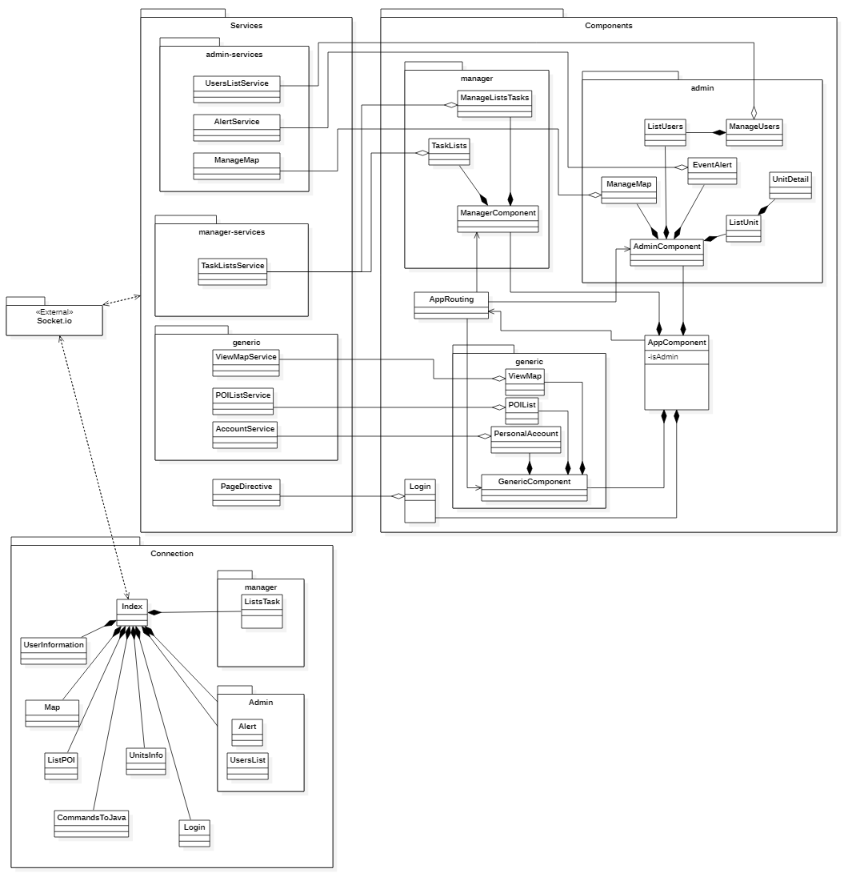
\includegraphics[scale=0.6]{res/images/UML_admin-manager.png}
	\caption{Diagramma UML delle classi per gli admin e i manager}
\end{figure}
Il diagramma di classe dell'admin-responsabile è molto simile a quello dell'unità: si avvale delle tecnologie Node, con il package connection, ed Angular, con tutti gli altri package.\\
Il contesto dei package è lo stesso dell'unità, di cui però si fa una differenziazione tra le funzionalità del'admin e quelle del manager grazie alla classe Login e al routing di AppRouting presente nel package component: permette all'utente di effettuare il login, "attivando" solamente le funzionalità riferite al tipo di utente loggato.\\
Il package generic contiene classi di funzionalità condivise tra amnagere e admin.\\
Le classi presenti in component permettono di attivare certe classi riferite al package (e quindi alle funzionalità di uno specifico tipo di utente):
\begin{itemize}
	\item admin:
	\begin{itemize}
		\item ListUsers → aggiunta o rimozione di manager;
		\item EventAlert → visualizzazione eventi eccezionali;
		\item ManageMap → modifica la planimetria e le caratteristiche della mappa;
	\end{itemize}
	\item manager:
	\begin{itemize}
		\item TaskLists → visualizzazione delle liste di task;
		\item MangeListsTask → aggiunta, modifica e rimozione di liste di task;
	\end{itemize}
	\item generic (sia per admin che per manager):
	\begin{itemize}
		\item ViewMap e POIList → visualizzazione in real time di tutte le unità nel magazzino.
	\end{itemize}
\end{itemize}



